%!TeX root=../tese.tex
%("dica" para o editor de texto: este arquivo é parte de um documento maior)
% para saber mais: https://tex.stackexchange.com/q/78101/183146

% Vamos definir alguns comandos auxiliares para facilitar.

% "textbackslash" é muito comprido.
% \newcommand{\sla}{\textbackslash}

% Vamos escrever comandos (como "make" ou "itemize") com formatação especial.
% \newcommand{\cmd}[1]{\textsf{#1}}

% Idem para packages; aqui estamos usando a mesma formatação de \cmd,
% mas poderíamos escolher outra.
% \newcommand{\pkg}[1]{\textsf{#1}}

% A maioria dos comandos LaTeX começa com "\"; vamos criar um
% comando que já coloca essa barra e formata com "\cmd".
% \newcommand{\ltxcmd}[1]{\cmd{\sla{}#1}}

\chapter{Proposal and Preliminary Experiments}
\label{cap:proposal}

As discussed in the previous chapters, understanding how social networks
recommend content to users is central to the debate around the recent waves of
political polarization and radicalization that have been taking over many
developing and developed countries alike. There are many ways of exploring
recommender systems without examining their code, from simulating their behavior
after careful observation to directly collecting recommendation data, but most
of them allow us to examine only one perspective of the algorithm at work. This
means that studying a social network's recommendation technique has inherent
limitations.

Most of the algorithms currently employed by social media companies are trade
secrets. They are also subject to constant experimentation and tuning, which
might render worthless any research performed before an update to the algorithm,
no matter how carefull the design of the study was. YouTube, for example,
currently has over 2 billion monthly logged-in users (which is more people than
any country in the planet), but it makes no significant effort to clarify
changes made to the algorithm or even whether they fulfill their promisses of
reducing user exposure to radicalizing content. With more than 500 hours of
content being uploaded every minute, if 1\% of all videos can be considered
radicalizing and the algorithm can detect 99\% of them, that still leaves over
25.000 hours of brand new extremist content free to spread on the platform every
year. YouTube claims only a small fraction of its content is political in
nature, but that doesn't mean it is not enough to spread across the internet and
help radicalize users the world over. It is also worth noting that most of these
platforms' efforts are concentrated in their parent countries (usually the
United States), so, even if they actually try and remove extreme content, most
of the non-English-speaking world would still not be impacted by their policy
changes.

This leads right into the goal of the present report. The dissertation to be
presented as a result of this program aims to make a tangible contribution to
the field of recommender systems, specifically how their design might (or might
not) foster confinement dynamics in the ``phase space'' of recommendations. If
the main hypothesis is confirmed, this could mean that recommendation algorithms
always create ``filter bubbles'', suggesting ever more engaging videos about a
certain topic of interest to a user, and possibly sending them on a
radicalization spiral if that topic is related to politics or other contentious
subjects.

\section{Datasets}
\label{sec:datasets}

Before discussing any experiment, it is necessary to introduce the datasets used
to train the models. The main dataset explored in this report is MovieLens
\citep{harper_movielens_2015}, a well-known set of movie reviews that has been
featured in many recommender system tutorials for the past few years. The full
dataset, with 27,000,000 ratings applied to 58,000 movies, was enriched by
\citet{banik_movies_2017} with information about the movies' credits, metadata,
keywords, and links. In the end, because of technical limitations, the dataset
used here was sampled until 30,689 movies were left; this allowed for faster
experimentation and simpler plots.

The second dataset, used for validation purposes only, was the Book-Crossing
Dataset \citep{ziegler_book-crossing_2004}. Just like the enriched MovieLens,
this dataset contained entries for ratings (1,149,780) applied by users
(278,858) to items (271,379 books), and information about these items like
title, author, publisher, etc.

\section{Experiments}
\label{sec:experiments}

Some preliminary experiments have already been conducted in order to gather some
evidence in favor or against the main hypothesis being tested. In total, fifteen
different recommendation models were trained and analyzed, with each plot below
representing one of these models. For simplicity's sake, even though all models
represented here are non-parametric, we still say they were ``trained'' because
the datasets used to generate recommendations are different.

The goal of these experiments was trying to identify if even a simple
recommendation algorithm could demonstrate some sort of bias towards a subset of
the items being recommended. More specifically, given an algorithm that cannot
be influenced by users' personal preferences, would the resulting recommender
system favor some kind of item? Excluding user information is important because,
as demonstrated by \citet{stoica_algorithmic_2018}, users might have their own
biases and these would get transferred on to the model; the objective here is
understanding the algorithm by itself without external influences.

To evaluate the recommendation models, at least qualitatively, the authors
plotted their ``recommendation profiles'': a summary of how many times an
arbitrary item is recommended overall. To create this profile, the algorithm is
asked to return the top-$n$ most similar items to the input according to its
internal similarity metric, and this process is repeated for every item in the
dataset. The recommendation profile of the model is the number of times each
item showed up in the top-$n$ most similar items of the whole dataset.

For example, a recommendation algorithm trained on the present version of the
MovieLens dataset would generate a list of $n$ movies for each input, creating a
list of $30,689 \times n$ movies. After this computationally intensive calculation,
the occurrence of each ID would be counted and ranked accordingly to facilitate
interpretation of results, that is, the movie ranked number 1 would be the movie
featured the most times in the set of all recommendations, and so forth for
every other rank. From now on, $n$ will be fixed to 10.

\begin{figure}
  \centering
  \begin{subfigure}{0.45\textwidth}
    \centering
    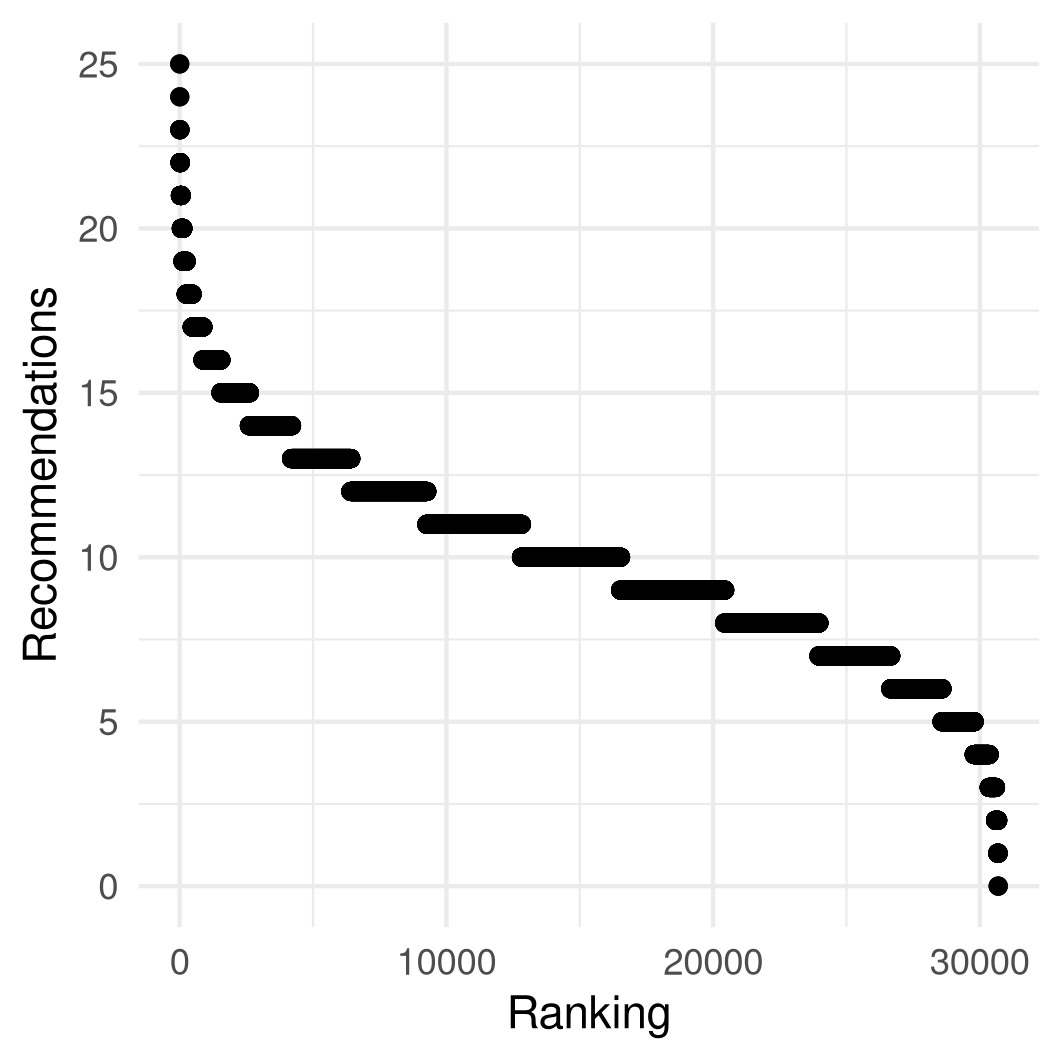
\includegraphics[width=\textwidth]{1a_random}
    \caption{Trivial recommendations.\label{fig:fig1a}}
  \end{subfigure}
  \begin{subfigure}{0.45\textwidth}
    \centering
    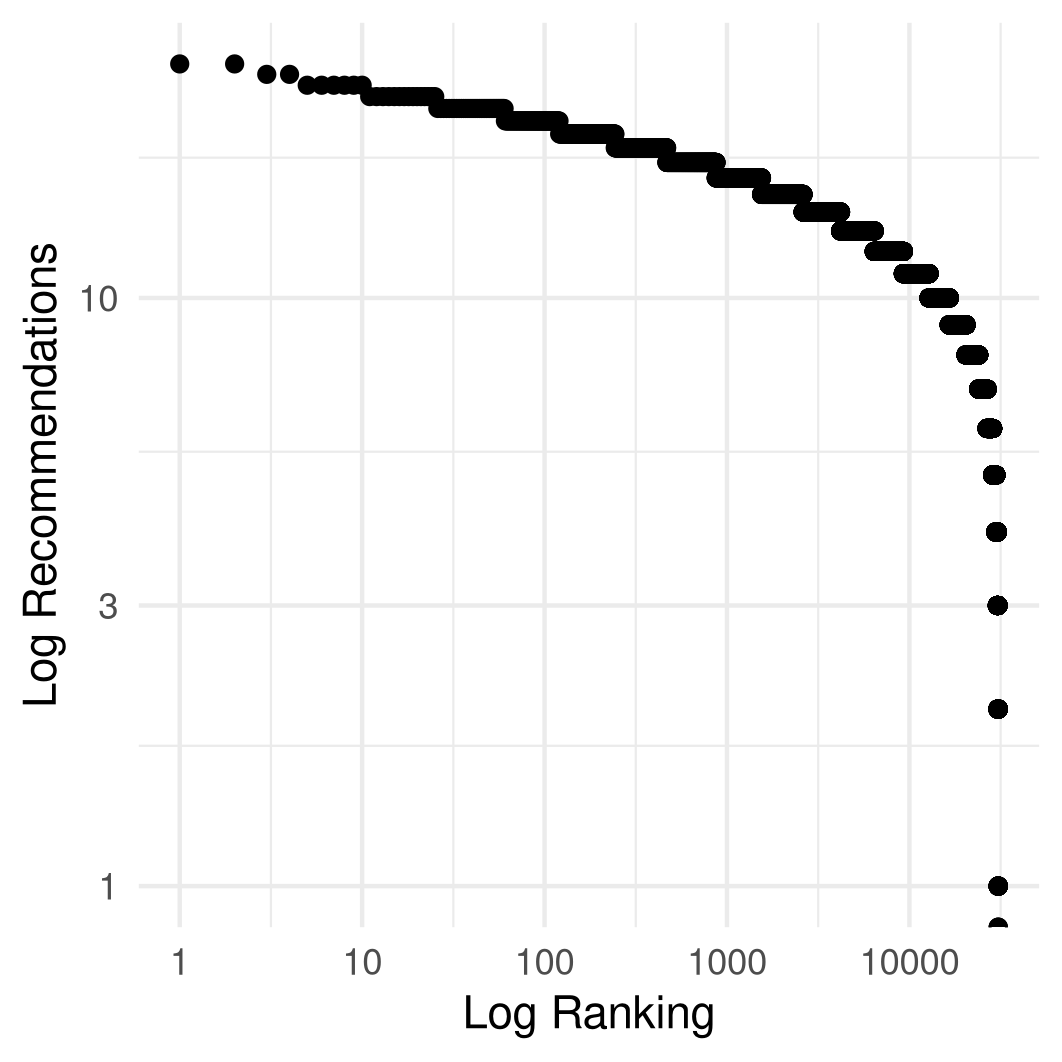
\includegraphics[width=\textwidth]{1b_random_log}
    \caption{Log-log plot.\label{fig:fig1b}}
  \end{subfigure}
  \caption{Recommendation profile for the trivial model (a) and log-log plot
    (b).\label{fig:fig1}}
\end{figure}

The baseline against which all models will be compared can be seen in
Figure~\ref{fig:fig1}, the so called ``trivial model''. This model is a simple
sampler that returns $n$ movies at random when asked for a recommendation and,
thus, its recommendation profile averaged, evidently, $n$, with an appearance
very similar to that of the CDF of the normal distribution. The ``most
recommended'' movie appeared 25 times in the final list, while the ``least
recommended'' movie did not appear at all. The log-log plot
(Figure~\ref{fig:fig1b}), despite seeming out of place, will make sense when the
second model is presented.

Besides the trivial model, the simplest model that excludes user information is
the content-based recommender. In the real world this is an algorithm that is
able to identify similar items based on their metadata (description, tags, etc.)
and suggest the closest items to the one being purchased or viewed. A
straightforward way of building such an algorithm is creating a vector
representation of each item and then using a similarity metric to recommend the
items most similar to the one in question. The chosen similarity metric was
cosine similarity because of its simplicity, robustness, and ubiquity
\citep{sarwar_item-based_2001}.

The main non-trivial model used in this study was the one that simply generated
vector representations for the full MovieLens dataset, without any modifications
(which is why it will henceforth be referred to as the ``vanilla'' model). The
metadata for each movie was made up of its keywords, main cast, director, and
genres. The vector transformation was very simple, with each position
representing one of the words of the corpus, and each element indicating how
many times that word appeared in the metadata for that movie. When the
recommendation for a movie was requested, the algorithm measured the cosine
similarity between it and every other movie, returning the IDs belonging to
the top $n = 10$ most similar vectors.

\begin{figure}
  \centering
  \begin{subfigure}{0.45\textwidth}
    \centering
    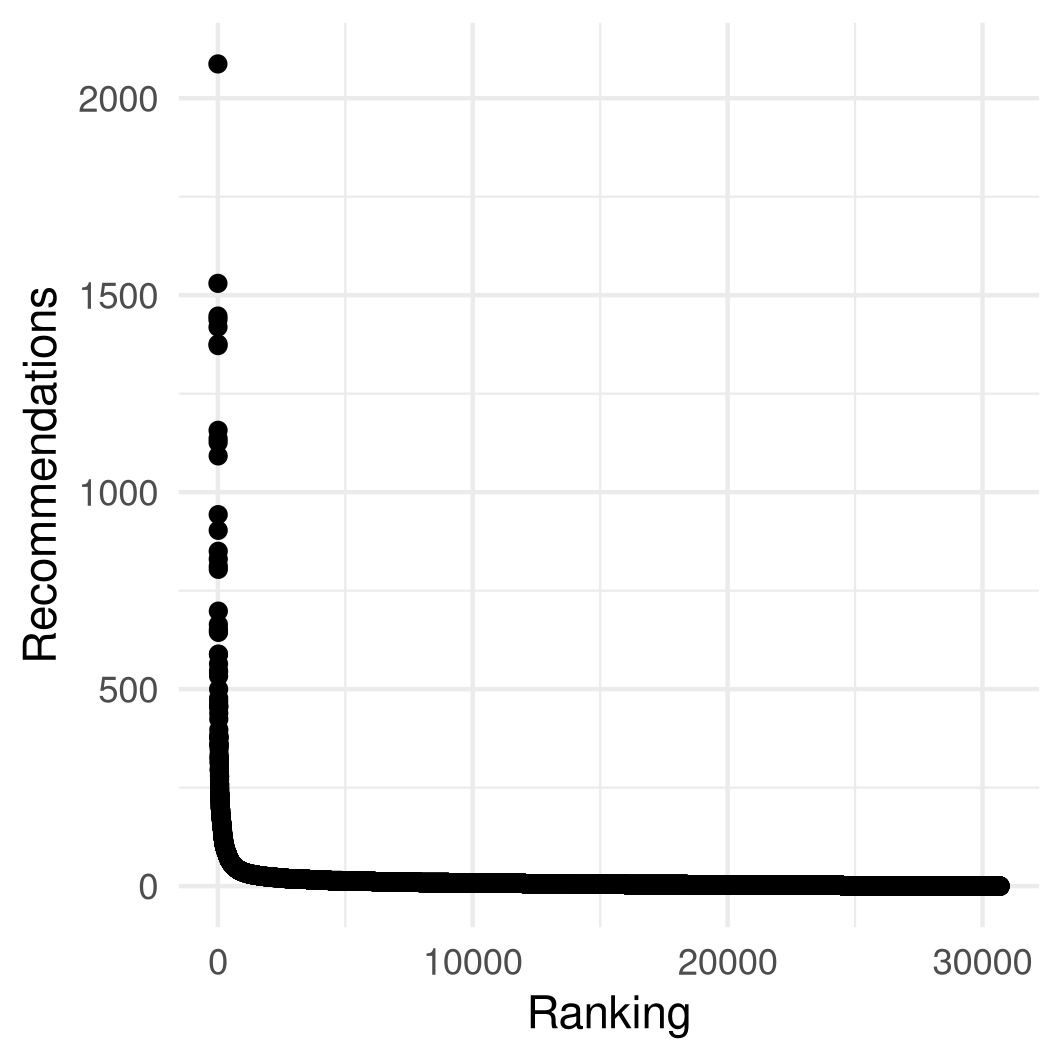
\includegraphics[width=\textwidth]{2a_vanilla}
    \caption{Rec. based on movie metadata.\label{fig:fig2a}}
  \end{subfigure}
  \begin{subfigure}{0.45\textwidth}
    \centering
    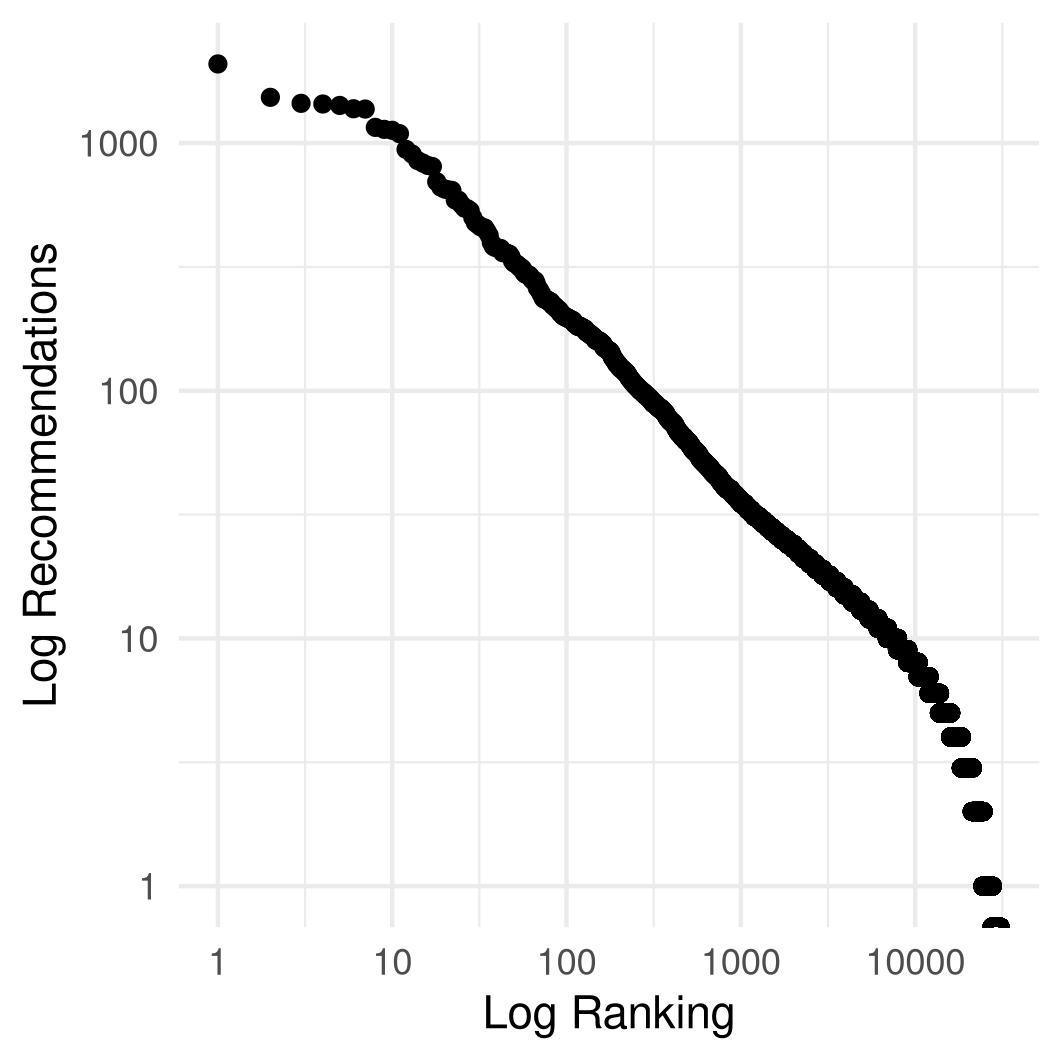
\includegraphics[width=\textwidth]{2b_vanilla_log}
    \caption{Log-log plot.\label{fig:fig2b}}
  \end{subfigure}
  \caption{Recommendation profile for the vanilla model (a) and log-log plot
    (b).\label{fig:fig2}}
\end{figure}

The recommendation profile for the vanilla model can be seen if
Figure~\ref{fig:fig2a}. Compared to Figure~\ref{fig:fig1a}, the same
visualization for the trivial model, the distribution of the vanilla model
differs immensely: the movie ranked number 1 appeared more than 2000 times in
the full list of recommendations, with an almost exponential decrease in the
number of appearances from then on. The log-log plots of both models
(Figure~\ref{fig:fig1b} and Figure~\ref{fig:fig2b}, respectively), makes it
clear that the vanilla model follows an exponential curve very closely, while
its trivial counterpart deviated in a major way.

\begin{figure}
  \centering
  \begin{subfigure}{0.3\textwidth}
    \centering
    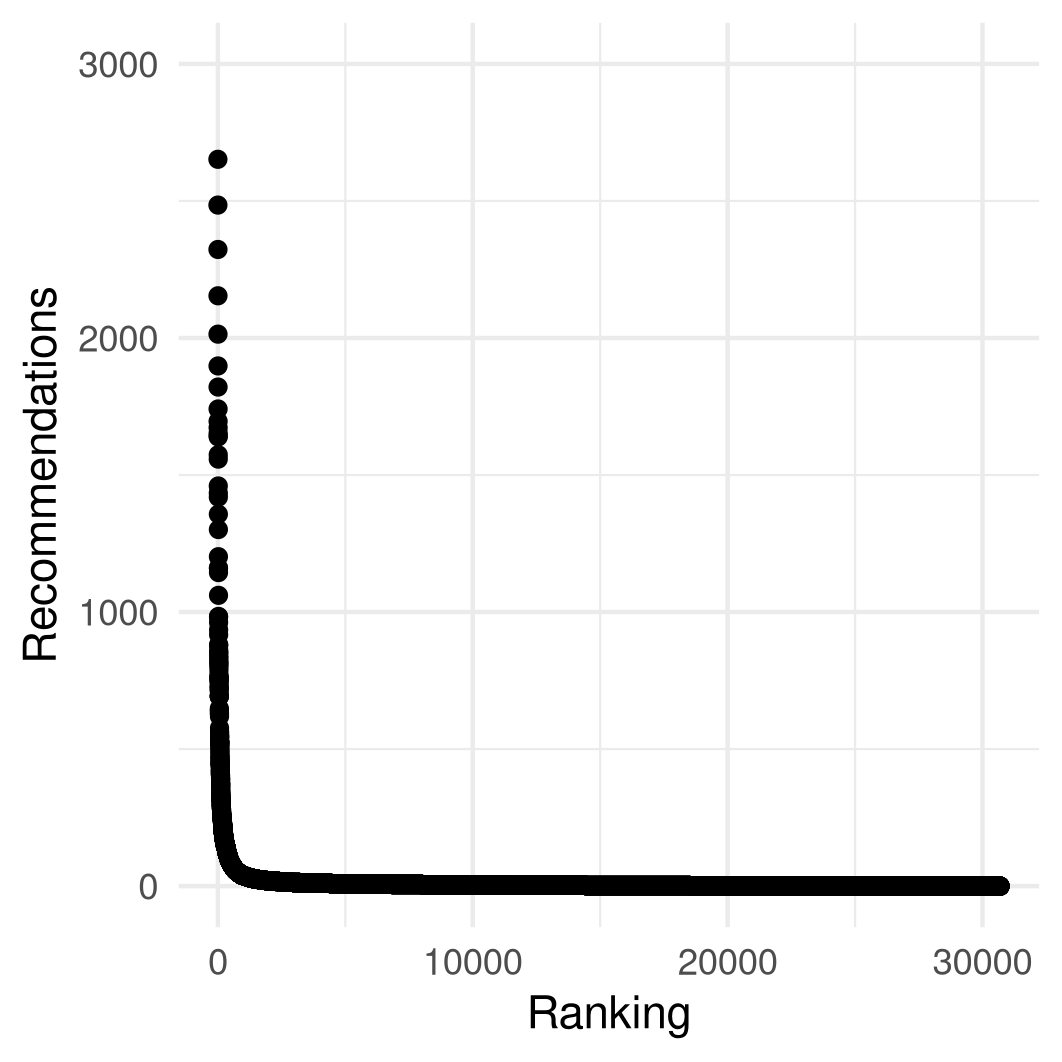
\includegraphics[width=\textwidth]{3a_cutoff_low}
    \caption{Cutoff $k = 2$.\label{fig:fig3a}}
  \end{subfigure}
  \begin{subfigure}{0.3\textwidth}
    \centering
    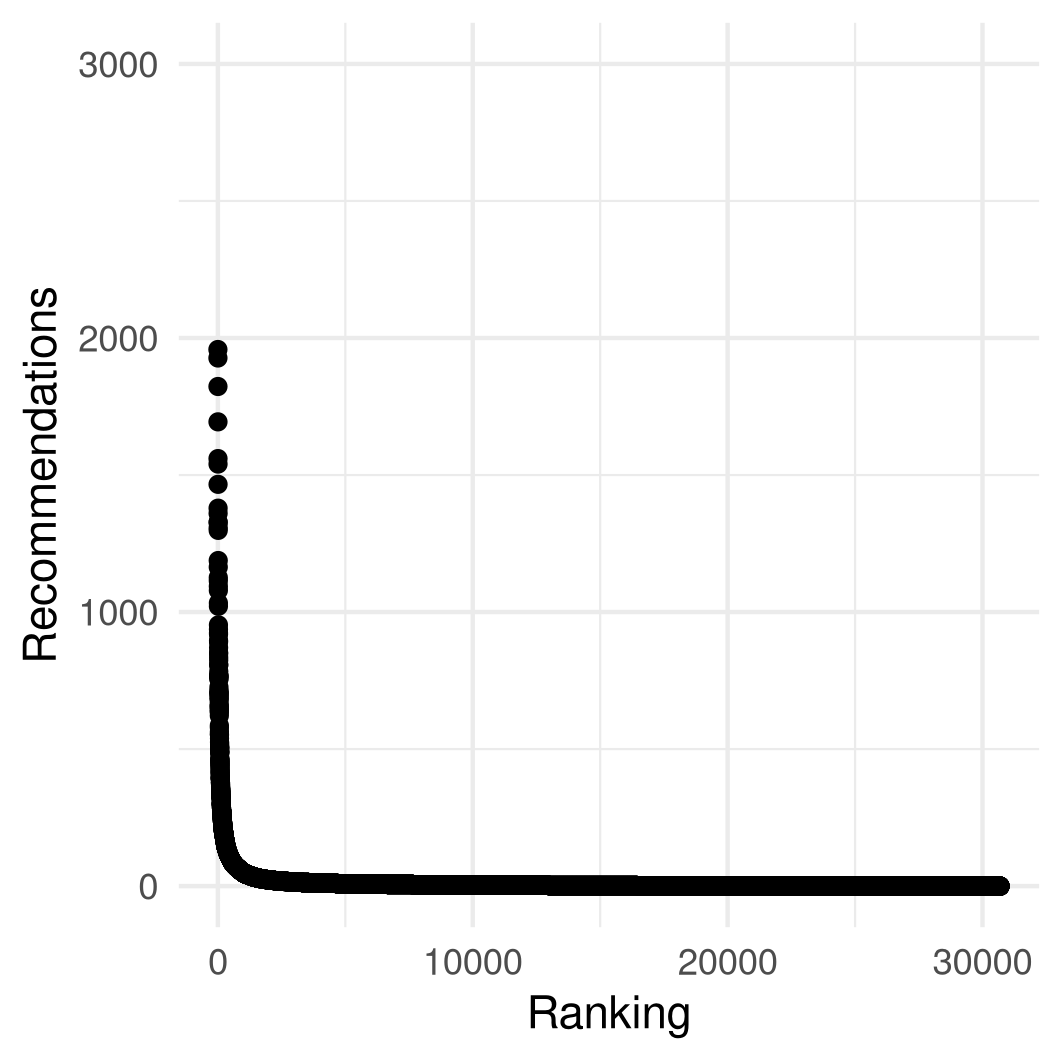
\includegraphics[width=\textwidth]{3b_cutoff_med}
    \caption{Cutoff $k = 5$.\label{fig:fig3b}}
  \end{subfigure}
  \begin{subfigure}{0.3\textwidth}
    \centering
    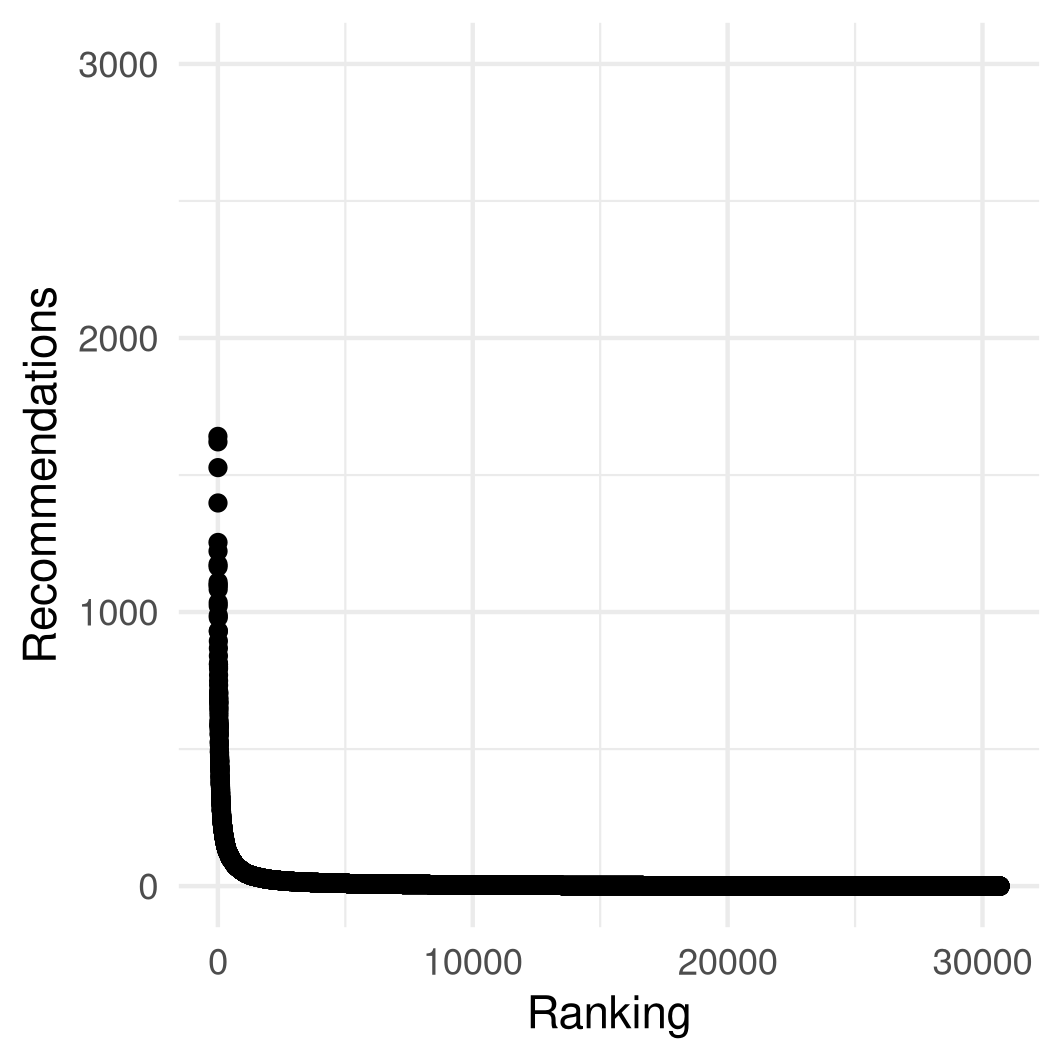
\includegraphics[width=\textwidth]{3c_cutoff_high}
    \caption{Cutoff $k = 8$.\label{fig:fig3c}}
  \end{subfigure}
  \caption{Recommendation profile for cutoff $k = 2$ (a), $5$ (b), and $8$
    (c).\label{fig:fig3}}
\end{figure}

A potential explanation for the difference between trivial and vanilla could
reside in the least used terms in the metadata: movies whose metadata share rare
words might have been recommended less frequently than movies whose metadata is
not so unique. To test this hypothesis, a cutoff point was created for words to
be included in the vector representation of the movies. Three cutoff points were
tested where only words with an absolute frequency larger than or equal to $k$,
$k = {2, 5, 8}$, could be included in the vector representations. The results
can be seen in Figure~\ref{fig:fig3} and, aside from variations in the
$y$-intercept, all plots are qualitatively very similar to
Figure~\ref{fig:fig2a}, indicating that rare words probably are not to blame for
the exponential decay.

\begin{figure}
  \centering
  \begin{subfigure}{0.3\textwidth}
    \centering
    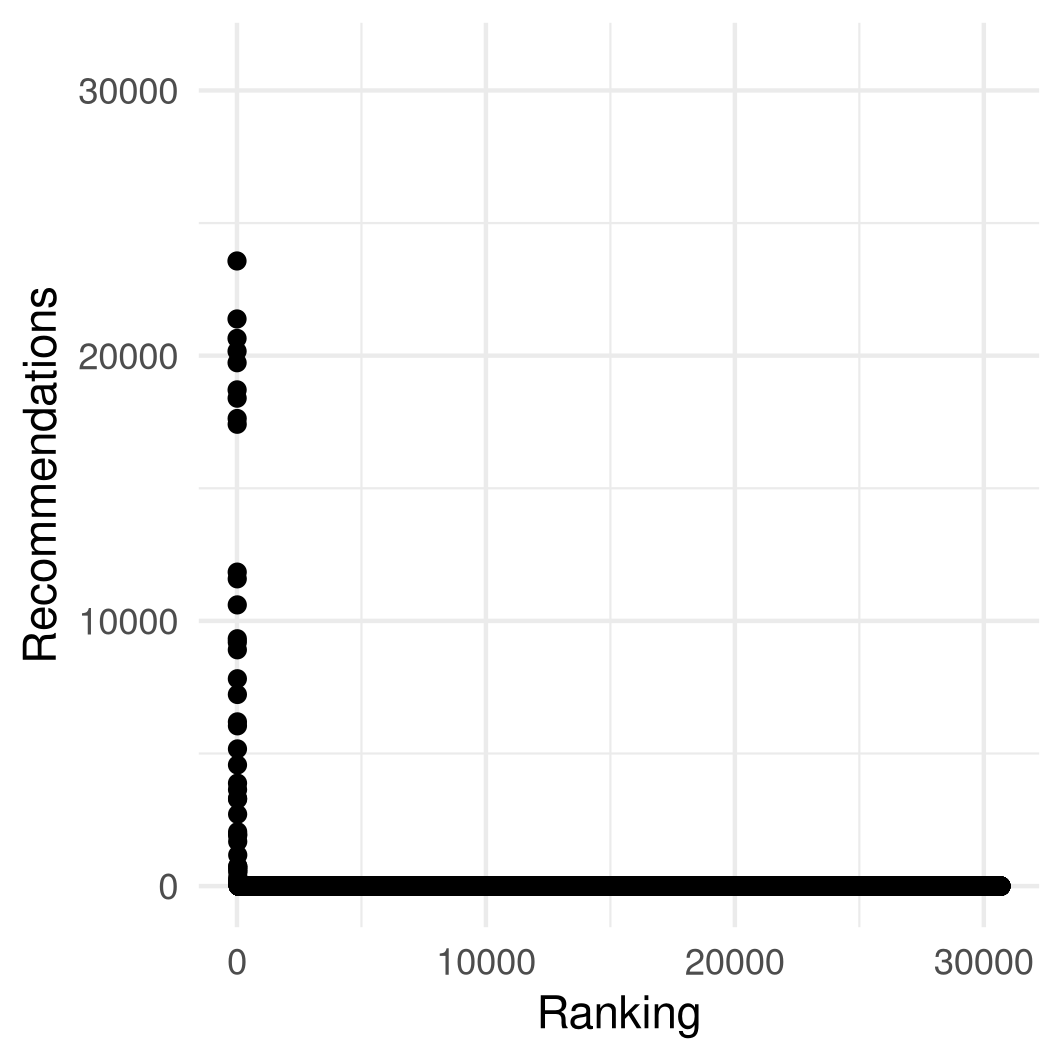
\includegraphics[width=\textwidth]{4a_cosine}
    \caption{Cosine distance.\label{fig:fig4a}}
  \end{subfigure}
  \begin{subfigure}{0.3\textwidth}
    \centering
    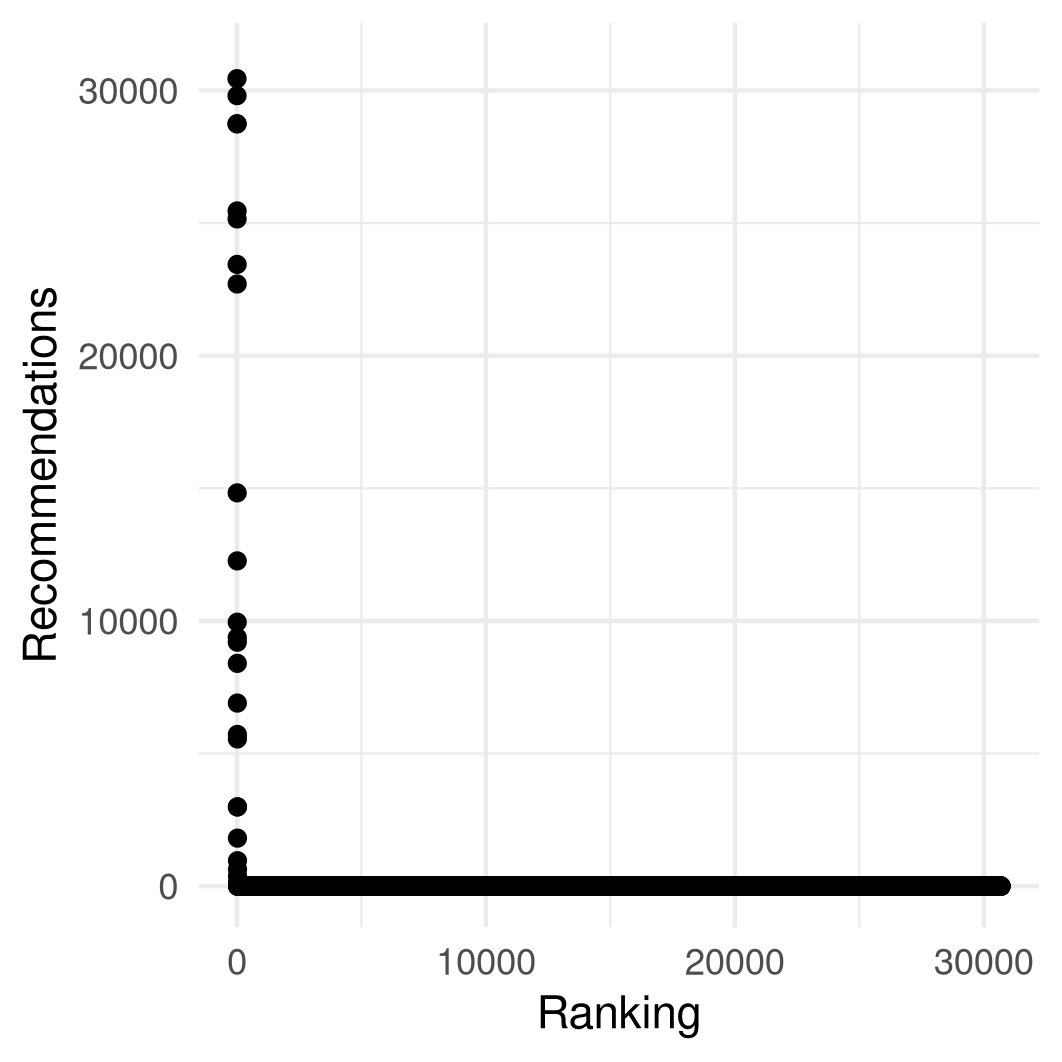
\includegraphics[width=\textwidth]{4b_euclidean}
    \caption{Euclidean distance.\label{fig:fig4b}}
  \end{subfigure}
  \begin{subfigure}{0.3\textwidth}
    \centering
    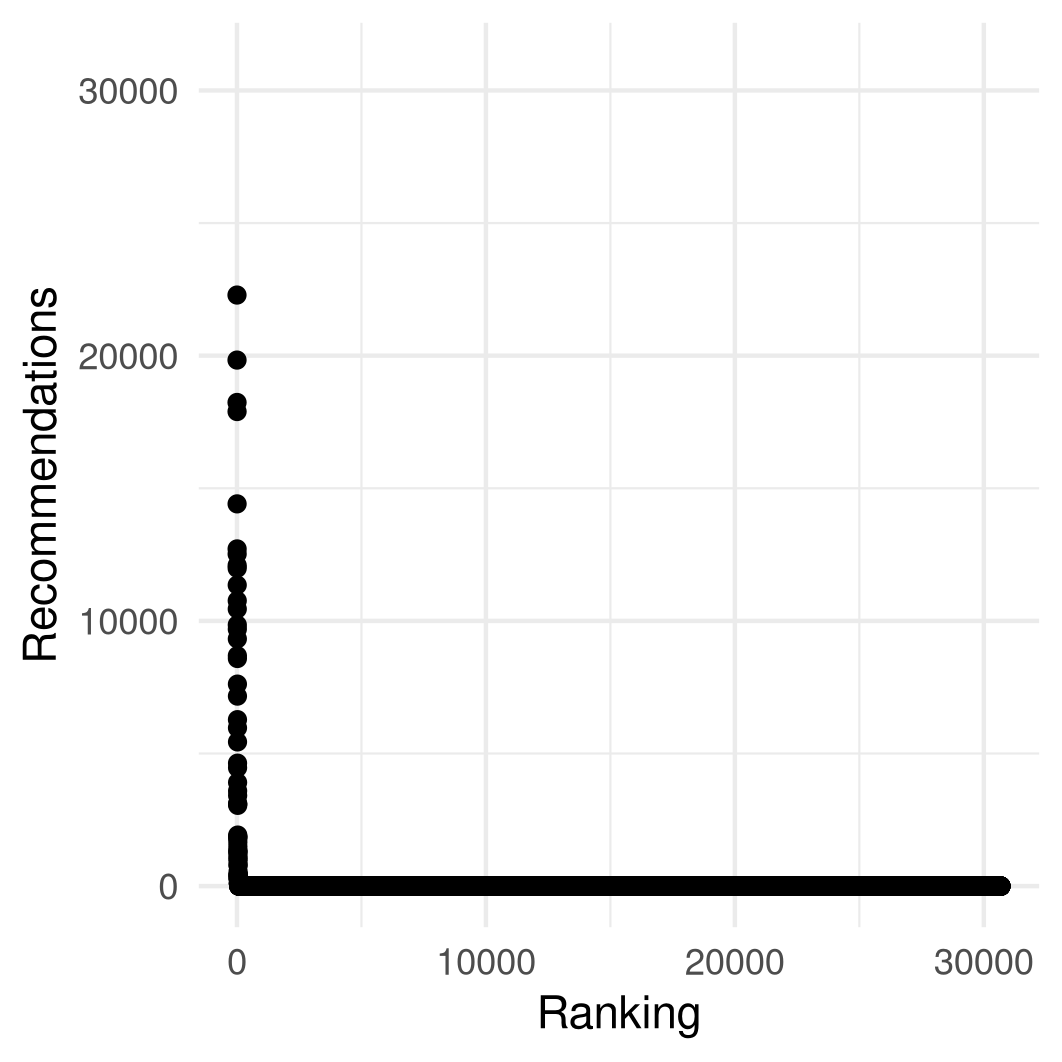
\includegraphics[width=\textwidth]{4c_manhattan}
    \caption{Manhattan distance.\label{fig:fig4c}}
  \end{subfigure}
  \caption{Recommendation profile for cosine (a), euclidean (b), and manhattan
    (c) distances.\label{fig:fig4}}
\end{figure}

The second validation experiment involved attempting to use other distance
metrics instead of cosine similarity \citep{ricci_introduction_2011}, since that
could also be a source of the strange behavior of the recommendation profile.
The goal here was verifying whether other metrics could do a better job at not
creating a subset of movies that ended up exponentially more recommended that
the rest. As attested by Figure~\ref{fig:fig4}, this was not the case. No other
similarity metrics were used because cosine seems to be the most popular one for
simple recommender systems. More experiments will be conducted comparing what
IDs belong to the group of top-recommended movies for each metric and if there
is intersection between them.

At this point it is safe to say that the exponential decay in recommendation
frequencies is not spurious and must have a clear cause. A hypothesis that is
later mostly confirmed involves the average number of non-zero elements in the
vector representation of the movies: the sparser the vectors, the higher the
odds of the recommendation curve displaying a steep left-hand side. This would
be almost equivalent to creating an ``inverse cutoff point'', removing common
words from the vector representations.

\begin{figure}
  \centering
  \begin{subfigure}{0.3\textwidth}
    \centering
    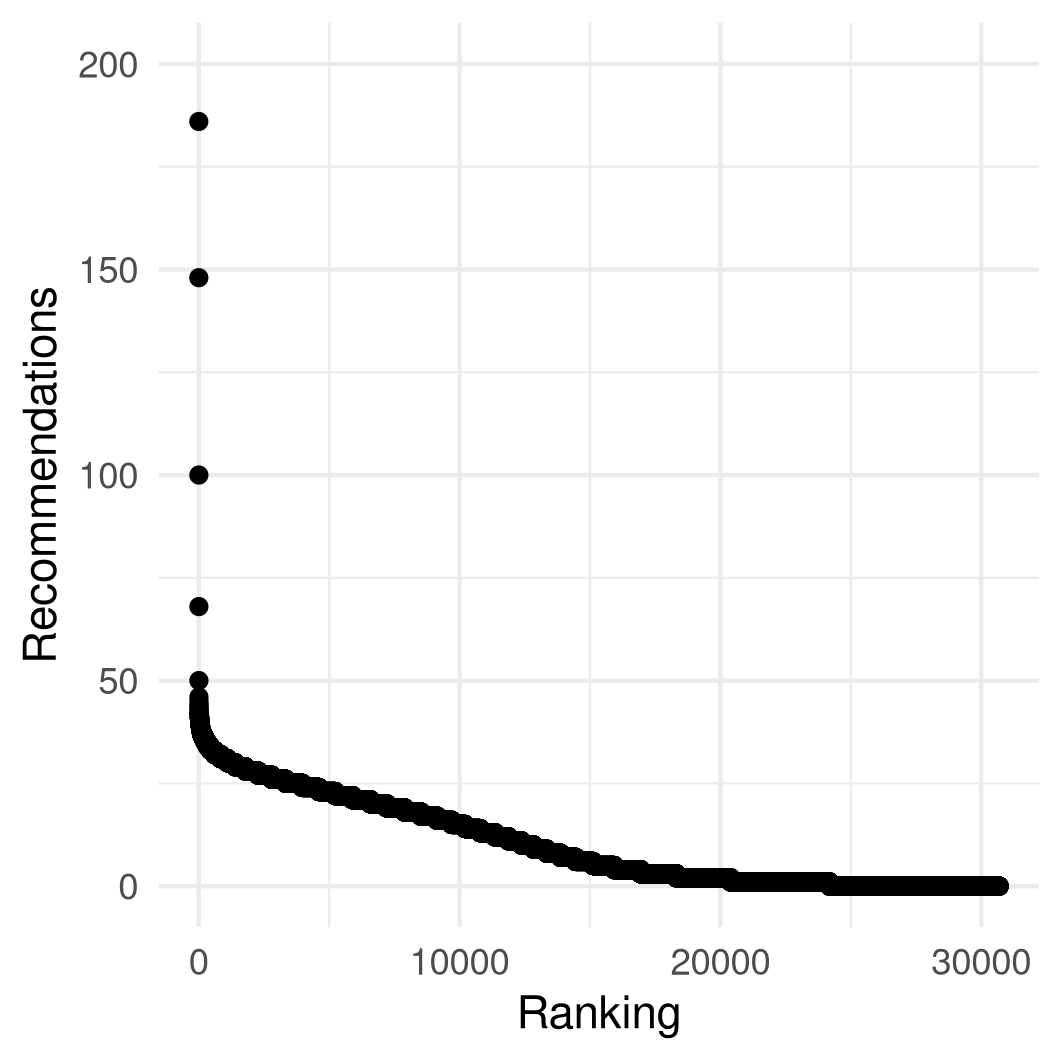
\includegraphics[width=\textwidth]{5a_p}
    \caption{$P(w_{i}) = 1 \times \overline{P(w)}$.\label{fig:fig5a}}
  \end{subfigure}
  \begin{subfigure}{0.3\textwidth}
    \centering
    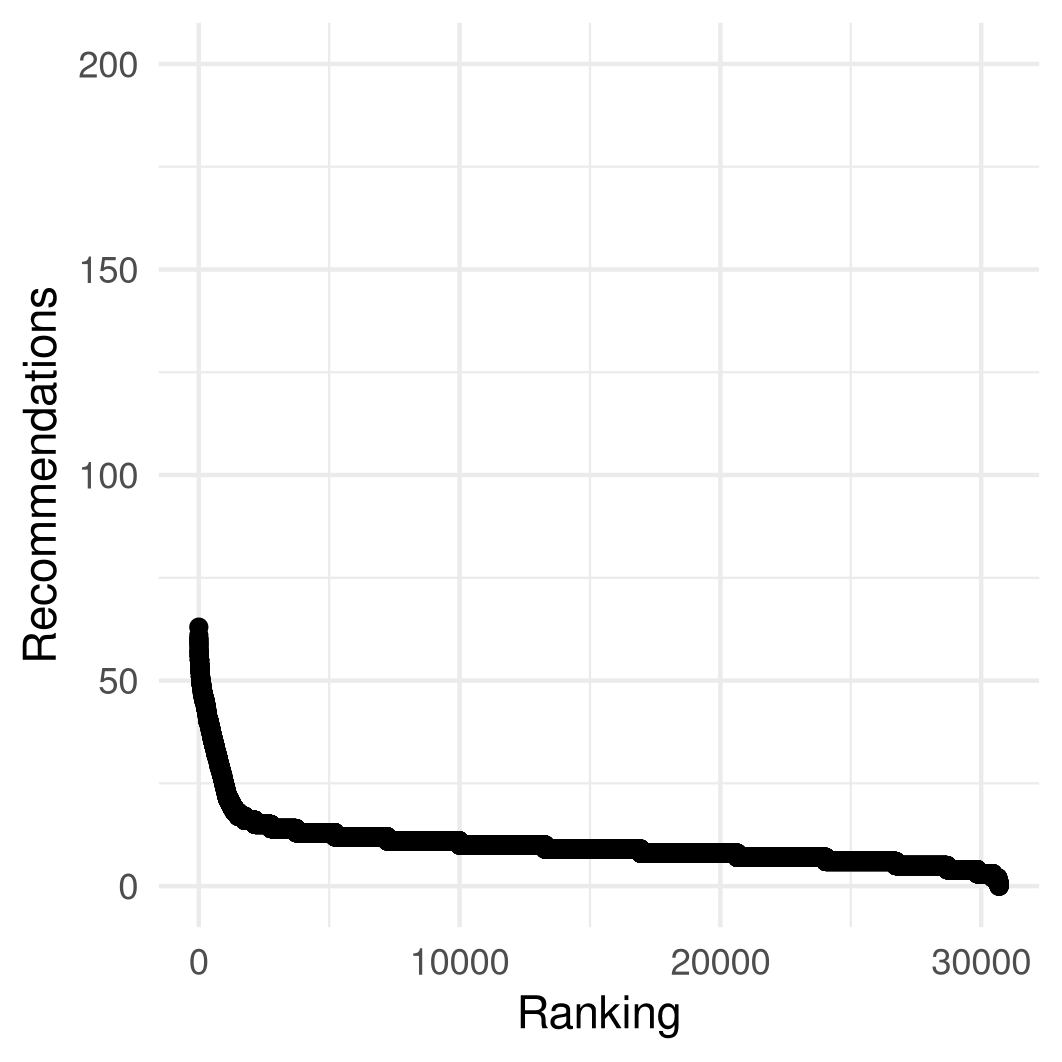
\includegraphics[width=\textwidth]{5b_p10}
    \caption{$P(w_{i}) = 10 \times \overline{P(w)}$.\label{fig:fig5b}}
  \end{subfigure}
  \begin{subfigure}{0.3\textwidth}
    \centering
    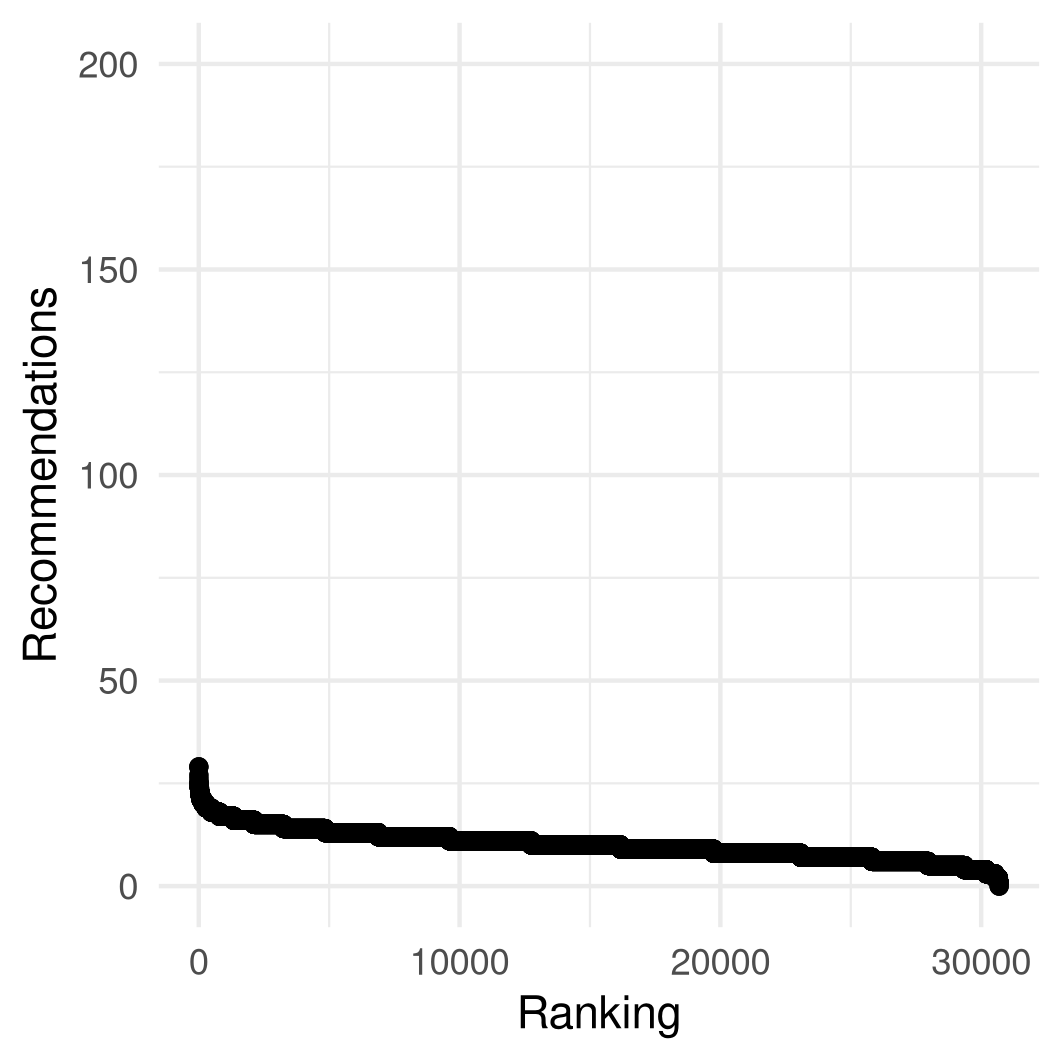
\includegraphics[width=\textwidth]{5c_p100}
    \caption{$P(w_{i}) = 100 \times \overline{P(w)}$.\label{fig:fig5c}}
  \end{subfigure}
  \caption{Recommendation profile of samples with
    $P(w_{i}) = C \times \overline{P(w)}$, $C = 1$ (a), $10$ (b), and $100$
    (c).\label{fig:fig5}}
\end{figure}

To test whether this hypothesis held water, ``random'' vector representations
were created. These representations were based on fictional metadata that were
comprised of words sampled at random from the full corpus of movies; the
probability that word $w_{i}$ occurred in the metadata of a fictional movie was
equal to the average probability that any word would occur in some arbitrary
metadata ($\overline{P(w)}$) times a costant $C$, $C = {1, 10, 100}$. More
simply, the probability of an element being non-zero in a random vector
representation was the average probability that an arbitrary element of the
vanilla representations was non-zero times $C$. The constant was added as a way
to create less sparse vectors and allow for comparisons between different
inverse cutoff points.

Figure~\ref{fig:fig5} displays the recommendation profiles for each different
$C$. Concretely, the figures are equivalent to creating random metadata for the
movies where the probability of a word occurring was approximately
$1.54 \times 10^{-4}$, $1.54 \times 10^{-3}$, and $1.54 \times 10^{-2}$ respectively and then
training the recommendation models. The results do support the aforementioned
hypothesis since less sparse vectors indeed generated less exponential decays.

\begin{figure}
  \centering
  \begin{subfigure}{0.45\textwidth}
    \centering
    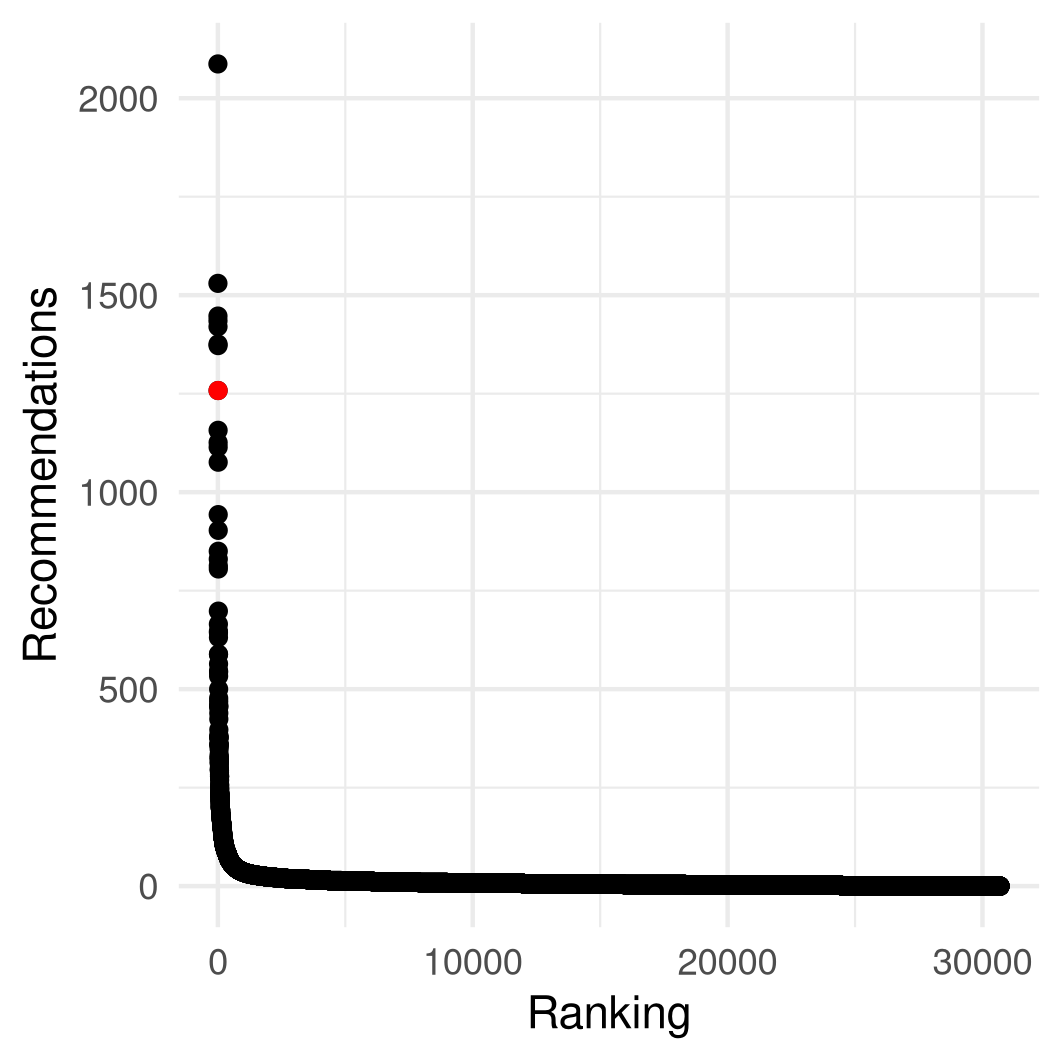
\includegraphics[width=\textwidth]{6a_artificial_movie}
    \caption{Vanilla model with artificial movie in red.\label{fig:fig6a}}
  \end{subfigure}
  \begin{subfigure}{0.45\textwidth}
    \centering
    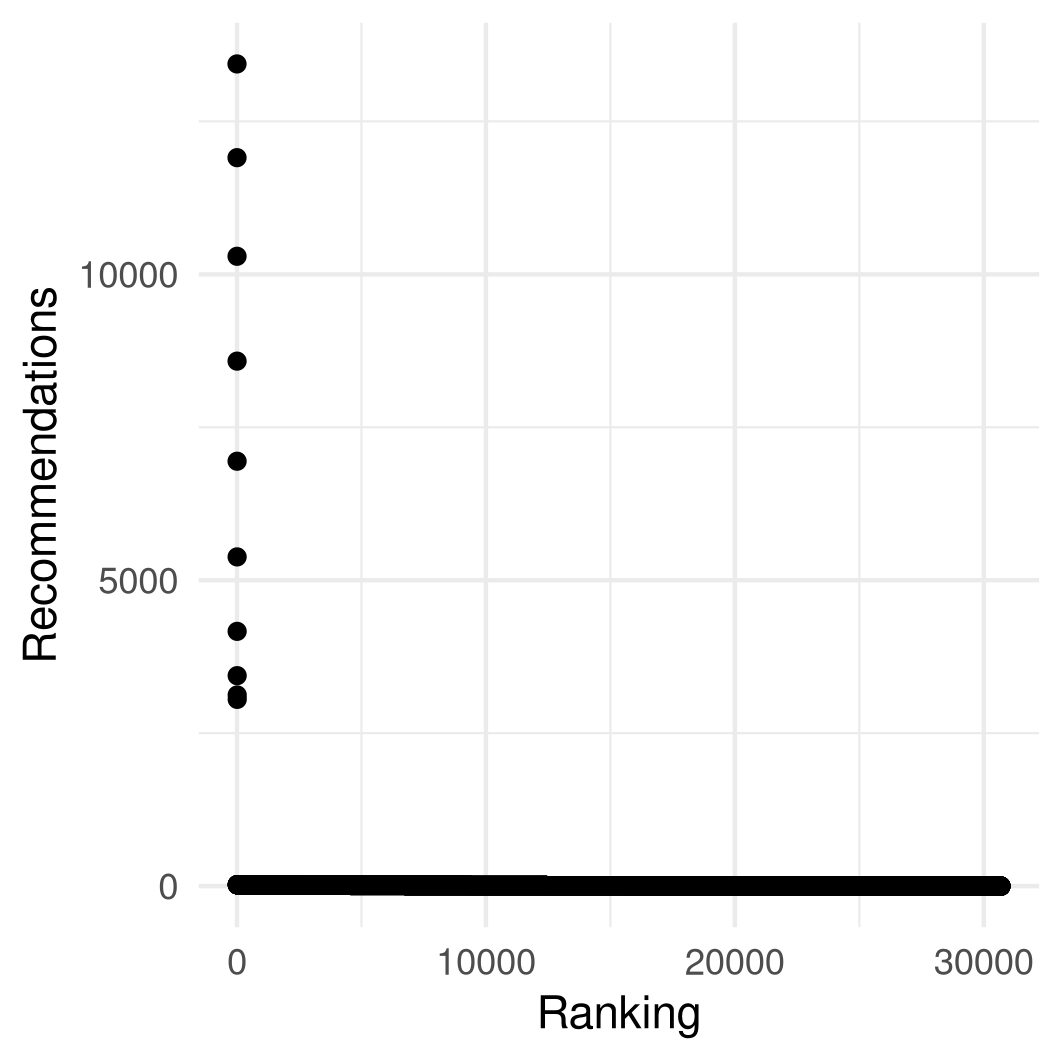
\includegraphics[width=\textwidth]{6b_long}
    \caption{Model with short vector representations.\label{fig:fig6b}}
  \end{subfigure}
  \caption{Recommendation profile for artificial movie (a) and short vector
    representations (b).\label{fig:fig6}}
\end{figure}

After the previous experiments, sanity checks were needed in order to guarantee
that the previous hypothesis was able generalize. The first check should verify
whether an artificial movie created as a combination of the metadata from other
movies favored by the recommendation algorithm would also be favored, while the
second should check whether shorter vectors would change the exponential decay
already observed despite being as sparse as their longer counterparts.

Figure~\ref{fig:fig6} showcases two sanity checks. Figure~\ref{fig:fig6a} was a
model trained with the vanilla dataset with the addition of the movie
highlighted in red. As expected, this movie also showed up in the
top-recommended subset. Figure~\ref{fig:fig6b} comes from a model trained on
randomly generated vector representations in a similar fashion to the ones in
Figure~\ref{fig:fig5}, except each vector could only have 15,000 elements
instead of 55,681 (as with the vanilla model). The patter observed before
persisted, meaning that the hypothesis still stood.

\begin{figure}
  \centering
  \begin{subfigure}{0.45\textwidth}
    \centering
    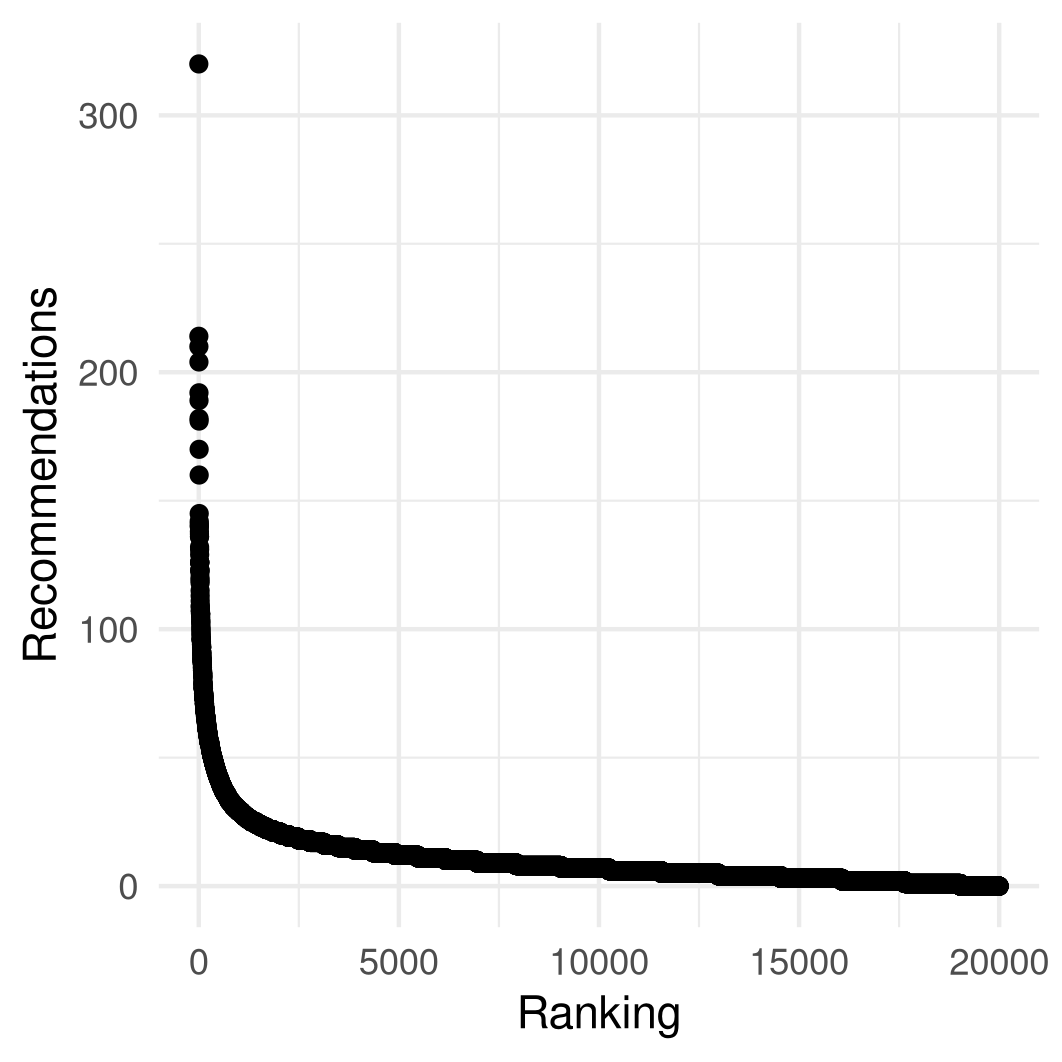
\includegraphics[width=\textwidth]{7a_books}
    \caption{Recommendation profile for book dataset.\label{fig:fig7a}}
  \end{subfigure}
  \begin{subfigure}{0.45\textwidth}
    \centering
    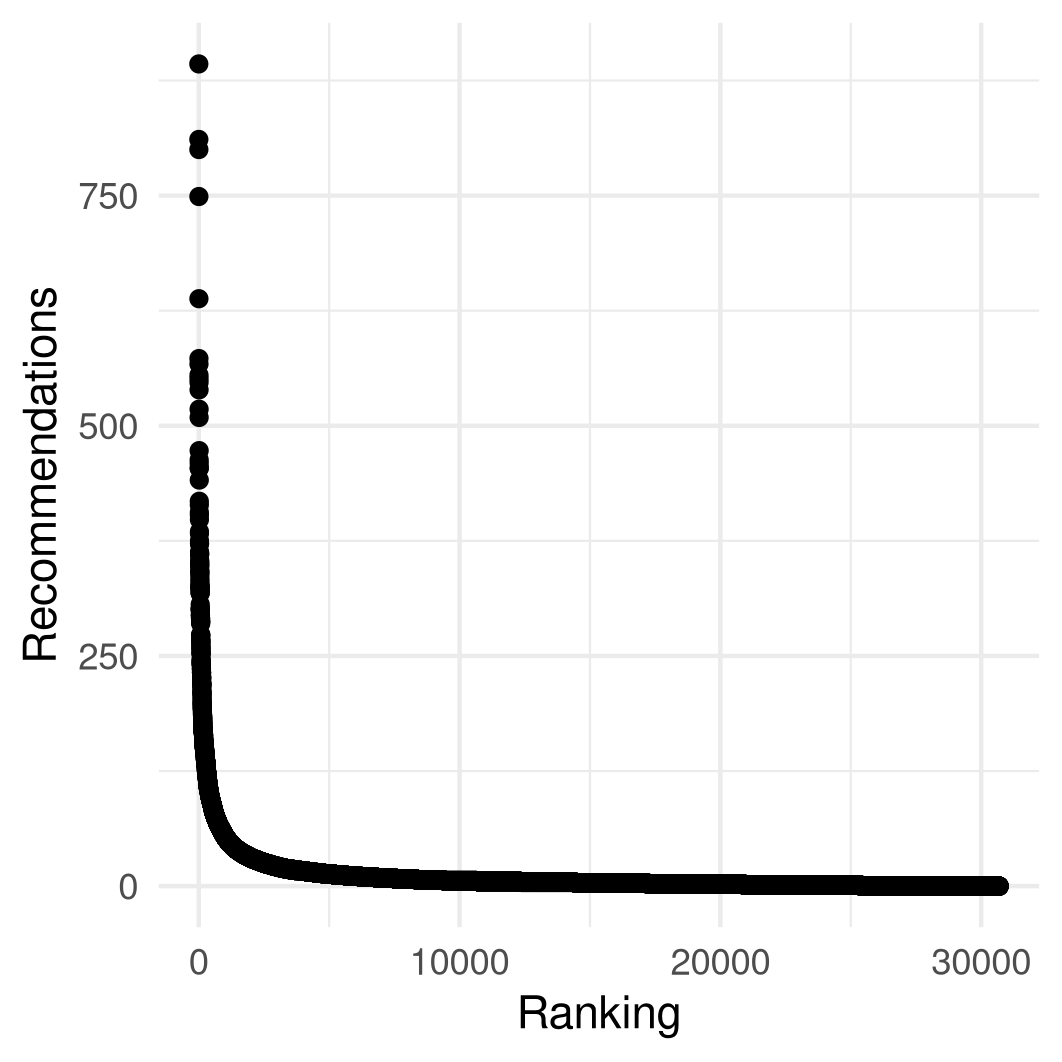
\includegraphics[width=\textwidth]{7b_mimic}
    \caption{Random simularion of vanilla.\label{fig:fig7b}}
  \end{subfigure}
  \caption{Recommendation profile for book dataset (a) and random simulation of
    vanilla (b).\label{fig:fig7}}
\end{figure}

The last two models were considered the confirmations of the hypothesis that
(at least for this kind of recommendation systems) a subset of items was always
exponentially more recommended than the rest as long as the data was sparse.
Figure~\ref{fig:fig7a} represents the same recommendation algorithm applied to
another dataset, the Book-Crossing dataset. Figure~\ref{fig:fig7b} contains the
results of the model applied to another set of random vector representations,
this time with the probability of each element being non-zero respecting the
marginal distributions of the vanilla dataset. Again, the exponential decay
pattern persisted, only slightly less pronounced in the Book-Crossing case.

\section{Further Experiments and Schedule}
\label{sec:schedule}

As previously mentioned, more experiments are still necessary in order to
identify exactly what is the nature of the bias detected in the MovieLens study.
For example, it would be interesting to perform an analysis of what movies are
the most recommended in each case and whether the subset of top-recommended
movies is roughly consistent overall. Continuous study of the literature about
recommender systems would also be of great help in searching for possible
explanations to this phenomenon.

The most important experiment that hasn't yet been conducted regards the dynamic
nature of recommendation algorithms. Using Google's newly released TensorFlow
Recommenders library \citep{noauthor_tensorflow_nodate} it might be possible to
gather data about what happens to a system's recommendations as users follow (or
don't follow) its suggestions, specially when talking about deep learning models
used by social networks like YouTube. This is a significant departure from the
content-based models presented here and, if a similar recommendation profile can
also be detected for multi-criteria recommender systems on dynamic scenarios,
then the hypothesis ventilated in the section above would become even more
plausible.

Showing that that these algorithms are suggesting a subset of items
exponentially more than the rest could be one more piece evidence in favor of
the pipeline theory of radicalization or, more simply, in favor of the theory
that these social networks are creating filter bubbles that radicalize users.
Literature about this topic is still scarce, but every day new papers about the
effects that social media has on Democracy are being released, so following up
on popular publications is of the utmost importance.

\begin{figure}
  \centering

  \begin{ganttchart}{2021-2}{2021-12}
    \gantttitlecalendar{year,month=shortname} \ganttnewline

    \ganttbar[progress=0]{Literature review}{2021-2}{2021-8} \ganttnewline
    \ganttbar[progress=0]{Algorithm implementation}{2021-3}{2021-6} \ganttnewline
    \ganttbar[progress=0]{Tests and experiments}{2021-4}{2021-7} \ganttnewline
    \ganttbar[progress=0]{Writing dissertation}{2021-5}{2021-9} \ganttnewline
    \ganttbar[progress=0]{Proofreading}{2021-8}{2021-10} \ganttnewline

    \ganttmilestone{Dissertation submission}{2021-10} \ganttnewline

    \ganttbar[progress=0]{Writing conference paper}{2021-10}{2021-12}
  \end{ganttchart}

  \caption{Schedule.\label{fig:gantt}}
\end{figure}

These two main tasks, alongside writing the final dissertation, will be the
focus of the coming semester. A full schedule can be seen in
Figure~\ref{fig:gantt}.
